\documentclass{pset}
\usepackage{tikz}
\usepackage{subcaption}

\psnum{3}
\psname{}
\psdue{See \cms{}}
\versionnumber{1}

\newcommand{\athree}{A3}
\newcommand{\afive}{A5}
\newcommand{\dfs}{Depth First Search}
\newcommand{\abutt}{\java{AbstractButterfly}}
\newcommand{\butt}{\java{Butterfly}}
\newcommand{\cms}{the CMS}

\begin{document}
\maketitle

%%%%%%%%%%%%%%%%%%%%%%%%%%%%%%%%%%%%%%%%%%%%%%%%%%%%%%%%%%%%%%%%%%%%%%%%%%%%%%%%
\section*{Overview}
In \athree{}, you will implement a boustrophedonic implementation of
\java{learn()}. From the Greek bous meaning ``ox'' and strephein meaning ``to
turn'', ``boustrophedonic'' literally translates to ``turning as an ox in
plowing''. A boustrophedonic search of a map uses the pattern of an ox plowing
a field: back and forth, alternating between west-to-east and east-to-west.

%%%%%%%%%%%%%%%%%%%%%%%%%%%%%%%%%%%%%%%%%%%%%%%%%%%%%%%%%%%%%%%%%%%%%%%%%%%%%%%%
\section*{Installation}
The following instructions walk you through the installation and setup of
Danaus' source code. If you do everything correctly, Eclipse should resemble
Figure~\ref{fig:eclipse}.
\begin{enumerate}
  \item Open a browser and navigate to the \athree{} page of \cms{}.
  \item Download \filename{Danaus.jar} and store it somewhere safe within your
    file system. Likely, the download will be in a Downloads directory. This
    works great.
  \item Open Eclipse.
  \item Select menu item \emph{File->New->Java Project}. A windowed menu will
    appear.
  \item Enter Danaus as the project name near the top of the window.
  \item Click \emph{Finish} near the bottom of the window.
  \item Select menu item \emph{File->Import}.
  \item Select \emph{General->Archive File} and click \emph{Next}.
  \item Click \emph{Browse\ldots} to the right of \emph{From archive file}
  \item  Navigate to \filename{Danaus.jar} that you previously stored on your
    hard drive. Select it and press \emph{OK}.
  \item  Click \emph{Finish}.
\end{enumerate}

\begin{figure}[h]
  \centering
  \includegraphics[width=0.5\textwidth]{img/eclipse}
  \caption{Eclipse after a correct installation of Danaus.}
  \label{fig:eclipse}
\end{figure}

%%%%%%%%%%%%%%%%%%%%%%%%%%%%%%%%%%%%%%%%%%%%%%%%%%%%%%%%%%%%%%%%%%%%%%%%%%%%%%%%
\part{Getting Started}
Before you begin implementing the boustrophedonic search, it may be helpful to
play around with Danaus and acclimate to its environment. This section provides
some brief suggestions of things to try with Danaus. If you already have a
strong familiarity with the system, feel free to ignore this section.

Let's begin with an empty implementation of \java{learn()}. It will look
something like this.

\begin{Java}
public TileState[][] learn() {return null;}
\end{Java}

Try running Danaus with this empty learn function. A windowed GUI should pop
up. The GUI should contain a graphical representation of a map and butterfly, a
slider to control the frame rate of the animation, information about the state
of the simulation, and information about the tile most recently clicked.

Now, let's begin flying. We can fly using function fly defined in
\java{AbstractButterfly}. \java{fly} takes in two parameters, \java{heading}
and \java{s}. \java{heading} is the direction in which you want your butterfly
to fly. \java{s} is the speed with which the butterfly will fly. Let's attempt
to fly east at a normal speed. Our learn method will now look like this.

\begin{Java}
public TileState[][] learn() {
    fly(danaus.Direction.E, danaus.Speed.NORMAL);
    return null;
}
\end{Java}

Now when you run Danaus, one of two things will happen.
\begin{enumerate}
  \item Your butterfly successfully flies east.
  \item Your butterfly collides with a cliff and throws and exception.
\end{enumerate}

Clearly, we do not want to prematurely terminate our program in the event of an
obstacle collision. We can remedy the situation by catching the exception. Our
learn method will now look like this.

\begin{Java}
public TileState[][] learn() {
	try {
		fly(danaus.Direction.E, danaus.Speed.NORMAL);
	}
	catch (danaus.CliffCollisionException e) {}
	return null;
}
\end{Java}

Now, our learn method safely attempts to fly east. In this contrived example,
we do not perform more than one fly operation, and we do not handle obstacle
collisions in a meaningful way. In this assignments and in future Danaus
assignments, your code will be much more complex.
\filename{RandomButterfly.java} contains a more complete demonstration of
flying.

%%%%%%%%%%%%%%%%%%%%%%%%%%%%%%%%%%%%%%%%%%%%%%%%%%%%%%%%%%%%%%%%%%%%%%%%%%%%%%%%
\part{Implement \java{learn()}}
We assume you have read through \filename{manual.pdf}. You can disregard
content that will be introduced in later assignments. You should have a basic
familiarity with Danaus, with \java{AbstractButterly}'s API, and with
\java{learn()}. Note the \java{learn()} you implement in \athree{} is slightly
different than the \java{learn()} you will implement later on in the course.

When \java{learn()} is called, your butterfly will be in the top left corner of
the map. It is your butterfly's responsibility to traverse the map in a
boustrophedonic fashion and construct a two-dimensional array of
\java{TileState}s to represent the portion of the map your butterfly explored.

Declare a two-dimensional array of \java{TileState}s of the appropriate size.
Get the height and width of the map using the appropriate functions in
\abutt{}.  

Next, have your butterfly travel east along the map using \java{fly()}.
Continue flying until the butterfly hits either the eastern edge of the map or
a cliff. Fly south one tile. Continue flying west until the butterfly once
again reaches either the western edge of the map or a cliff. Once again, fly
south one tile.  Repeat this process until one of three terminating conditions
is met.
\begin{enumerate}
  \item Your butterfly is in the bottom row of the map flying east, and it
    reaches the southeast corner of the map.
  \item Your butterfly is in the bottom row of the map flying west, and it
    reaches the southwest corner of the map.
  \item Your butterfly is in the bottom row of the map flying east or west and
    collides with a cliff.
\end{enumerate}

In \athree{}, we guarantee that your butterfly will unconditionally be able to
fly south in the event of a collision with a cliff or an edge of the map. 

Every time the butterfly enters a previously unexplored tile, use
\java{refreshState()} to retrieve its \java{TileState} and store it in the
appropriate spot of the two-dimensional array. A tile at row \java{r} and
column \java{c} should be stored in the array at row \java{r} and column
\java{c}. Use \java{state.location.row} and \java{state.location.col} to access
the row and column.  Once the butterfly has finished its search and the array
of \java{TileState}s has been properly constructed, return the array. This will
end the learning phase of the simulation.

Example boustrophedonic searches are given in Figure~\ref{fig:no-cliffs},
Figure~\ref{fig:cliffs}, and Figure~\ref{fig:min-horizontal}.

\section*{Grading}
We will grade your boustrophedonic search algorithm against the course staff's
implementation. The grading steps can summarized as follows.
\begin{enumerate}
  \item Generate map.
  \item Run your butterfly on the map and generate a two-dimensional array
    \java{M} of \java{TileState}s.
 \item Run our butterfly on the map and generate a two-dimensional array
   \java{M'} of \java{TileStates}. Compare \java{M} to \java{M'} and generate
   score.  If your array \java{M} matches \java{M'} exactly, you will receive a
   good score.  If \java{M} is different than \java{M'}, you will receive a
   score based on the similarity. 
\end{enumerate}

\section*{Checklist}
Before you submit your assignment, check to see that you have completed the
following tasks.
\begin{itemize}
  \item You have read this document and \filename{manual.pdf} in detail.
  \item You have read and agreed to the academic code of integrity. 
  \item If you have a partner, you have formed a group on \cms{}. This must be
    done before you submit.
  \item You have reviewed CS 2110's coding style guidelines, and your code
    adheres to the guidelines.
  \item The fields of \butt{} are annotated with the class invariant.
  \item Each method of \butt{} has a good javadoc specification.
  \item You have placed the total time spent on the assignment at the top of
    \filename{Butterfly.java}
\end{itemize}

\section*{Deliverables}
On \cms{}, submit the following files.
\begin{enumerate}
  \item  \filename{Butterfly.java}. This file contains subclass Butterfly,
    including your implementation of a boustrophedonic \java{learn()}.
\end{enumerate}

\begin{figure}[p]
  \centering
  \begin{subfigure}{0.45\textwidth}
    \centering
    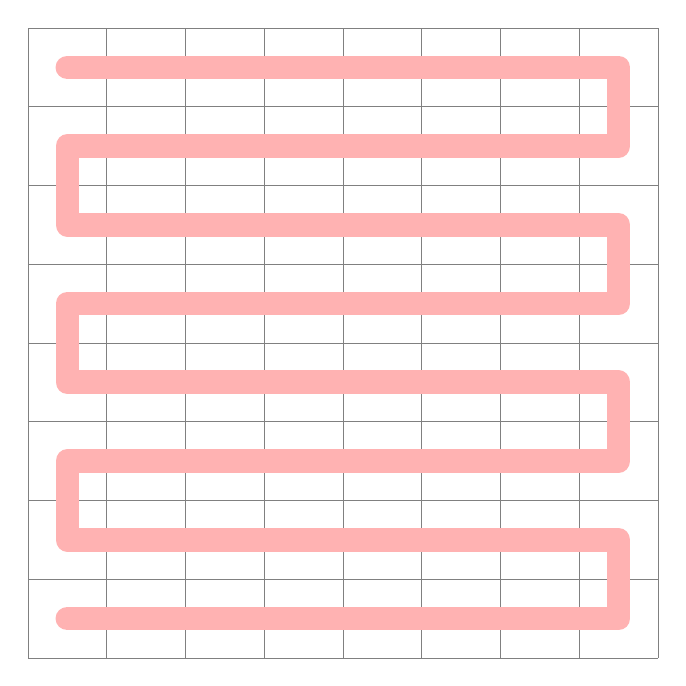
\begin{tikzpicture}
      \draw[help lines] grid (8.0,8.0);
      \draw[line width=0.3cm,color=red!30,cap=round,join=round] 
        (0.5, 7.5) --
        (7.5, 7.5) --
        (7.5, 6.5) --
        (0.5, 6.5) --
        (0.5, 5.5) --
        (7.5, 5.5) --
        (7.5, 4.5) --
        (0.5, 4.5) --
        (0.5, 3.5) --
        (7.5, 3.5) --
        (7.5, 2.5) --
        (0.5, 2.5) --
        (0.5, 1.5) --
        (7.5, 1.5) --
        (7.5, 0.5) --
        (0.5, 0.5);
    \end{tikzpicture}
    \caption{A boustrophedonic search on a map without cliffs.}
    \label{fig:no-cliffs}
  \end{subfigure} \quad\quad
  \begin{subfigure}{0.45\textwidth}
    \centering
    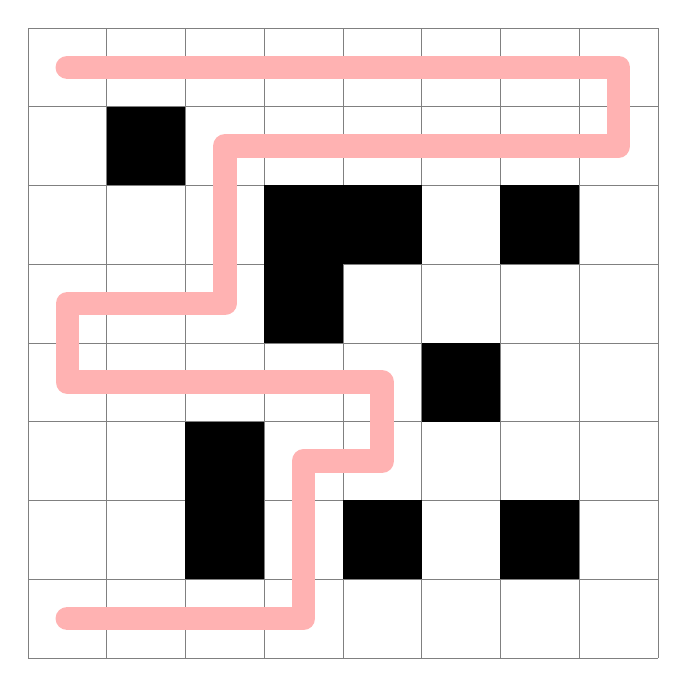
\begin{tikzpicture}
      \draw[help lines] grid (8.0,8.0);
      \fill[black] (1,6) rectangle (2,7);
      \fill[black] (3,5) rectangle (4,6);
      \fill[black] (4,5) rectangle (5,6);
      \fill[black] (6,5) rectangle (7,6);
      \fill[black] (3,4) rectangle (4,5);
      \fill[black] (5,3) rectangle (6,4);
      \fill[black] (2,2) rectangle (3,3);
      \fill[black] (2,1) rectangle (3,2);
      \fill[black] (4,1) rectangle (5,2);
      \fill[black] (6,1) rectangle (7,2);
      \draw[line width=0.3cm,color=red!30,cap=round,join=round] 
        (0.5, 7.5) --
        (7.5, 7.5) --
        (7.5, 6.5) --
        (2.5, 6.5) --
        (2.5, 4.5) --
        (0.5, 4.5) --
        (0.5, 3.5) --
        (4.5, 3.5) --
        (4.5, 2.5) --
        (3.5, 2.5) --
        (3.5, 0.5) --
        (0.5, 0.5);
    \end{tikzpicture}
    \caption{A boustrophedonic search on a map populated with cliffs.}
    \label{fig:cliffs}
  \end{subfigure}

  \begin{subfigure}{0.45\textwidth}
    \centering
    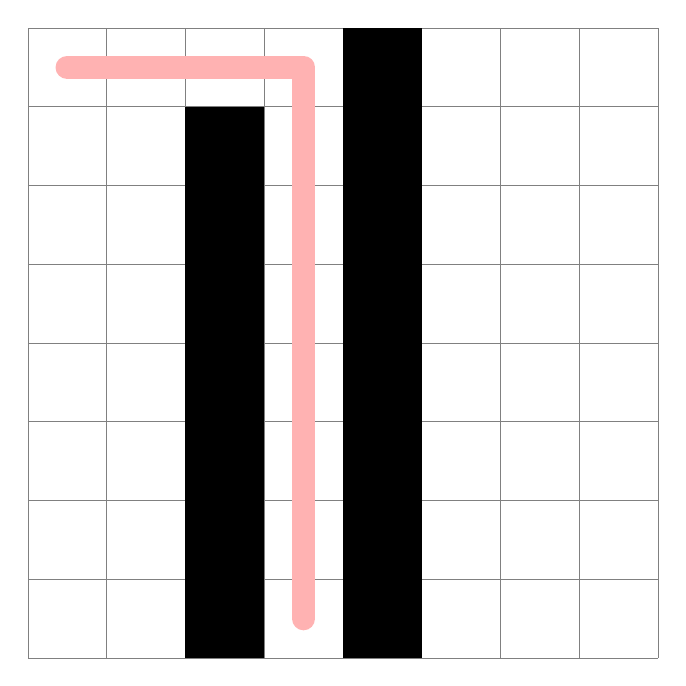
\begin{tikzpicture}
      \draw[help lines] grid (8.0,8.0);
      \fill[black] (2,0) rectangle (3,1);
      \fill[black] (2,1) rectangle (3,2);
      \fill[black] (2,2) rectangle (3,3);
      \fill[black] (2,3) rectangle (3,4);
      \fill[black] (2,4) rectangle (3,5);
      \fill[black] (2,5) rectangle (3,6);
      \fill[black] (2,6) rectangle (3,7);
      \fill[black] (4,0) rectangle (5,1);
      \fill[black] (4,1) rectangle (5,2);
      \fill[black] (4,2) rectangle (5,3);
      \fill[black] (4,3) rectangle (5,4);
      \fill[black] (4,4) rectangle (5,5);
      \fill[black] (4,5) rectangle (5,6);
      \fill[black] (4,6) rectangle (5,7);
      \fill[black] (4,7) rectangle (5,8);
      \draw[line width=0.3cm,color=red!30,cap=round,join=round] 
        (0.5, 7.5) --
        (3.5, 7.5) --
        (3.5, 0.5);
    \end{tikzpicture}
    \caption{A boustrophedonic search with minimal horizontal flight.}
    \label{fig:min-horizontal}
  \end{subfigure}
    
  \caption{Sample boustrophedonic searches}
  \label{fig:bsearches}
\end{figure}

\end{document}
